\documentclass[runningheads,a4paper]{llncs}

\usepackage{mathtools}
\usepackage{amssymb}
\setcounter{tocdepth}{3}
\usepackage{graphicx}
\usepackage{wrapfig}
\usepackage[caption=false]{subfig}
\usepackage{tikz}
\usepackage{pgfplots}
\pgfplotsset{compat=1.9}

\usepackage{url}
\usepackage{algpseudocode}
\usepackage{algorithm}
\usepackage{algorithmicx}


%\captionsetup[figure]{width=.85\textwidth}
%\captionsetup[subfigure]{width=.45\textwidth}
  
\newcommand{\keywords}[1]{\par\addvspace\baselineskip
\noindent\keywordname\enspace\ignorespaces#1}

%To economize paper
%\textwidth=190mm
%\textheight=250mm
%\topmargin=-20mm
%\oddsidemargin=-15mm
%\evensidemargin=-15mm


\begin{document}

\algnewcommand\algorithmicswitch{\textbf{switch}}
\algnewcommand\algorithmiccase{\textbf{case}}
\algnewcommand\algorithmicassert{\texttt{assert}}
\algnewcommand\Assert[1]{\State \algorithmicassert(#1)}
% New "environments"
\algdef{SE}[SWITCH]{Switch}{EndSwitch}[1]{\algorithmicswitch\ #1\ \algorithmicdo}{\algorithmicend\ \algorithmicswitch}
\algdef{SE}[CASE]{Case}{EndCase}[1]{\algorithmiccase\ #1}{\algorithmicend\ \algorithmiccase}

\algtext*{EndSwitch}
\algtext*{EndCase}
\algtext*{EndWhile}% Remove "end while" text
\algtext*{EndIf}% Remove "end if" text
\algtext*{EndFor}% Remove "end for" text
\algtext*{EndFunction}% Remove "end function" text

\newtheorem{mydef}{Definition}
\newtheorem{mytheorem}{Theorem}

\mainmatter  % start of an individual contribution


\title{Context-Free Language Reachability by Matrix Multiplication}

\titlerunning{CFL-reachability by Matrix Multiplication}

\author{Rustam Azimov \and Semyon Grigorev}
\authorrunning{Rustam Azimov, Semyon Grigorev}


\institute{ Saint Petersburg State University\\
            7/9 Universitetskaya nab.\\
            St. Petersburg, 199034 Russia\\
\email{\path|rustam.azimov19021995@gmail.com| }
\\
\email{\path|Semen.Grigorev@jetbrains.com|}
}


\toctitle{Context-Free Path Querying by Matrix Multiplication}
\tocauthor{Rustam Azimov}
\maketitle

%\tableofcontents


\begin{abstract}
	Problems in many areas, for example, bioinformatics, graph databases, program analysis, can be reduced to one of the graph reachability problems where some paths in the given directed edge-labeled graph are specified using formal grammars over the alphabet of edge labels. One of the most popular formulations of this problem is the \textit{all-pairs} context-free language (CFL) reachability. For this formulation, it is necessary to compute a set of pairs $(m, n)$ such that there is a path from node $m$ to node $n$, whose labeling is generated by the given context-free grammar. There are a number of algorithms in dynamic-programming style for solving the all-pairs CFL-reachability but all of them perform poorly on large graphs. One of the open problems in this area is to generalize a well-known matrix-based context-free recognition solution (Valiant 1975) to solve the all-pairs CFL-reachability problem. In this paper, we show how the all-pairs CFL-reachability problem can be reduced to the calculation of the matrix transitive closure. Also, we propose a matrix-based algorithm for solving this problem.

\keywords{Context-free language reachability, context-free grammar, transitive closure, matrix multiplication}
\end{abstract}


\section{Introduction}%--------------------------------------------------------------------------------------------------------------------------------------------
Problems in many areas, for example, bioinformatics~\cite{Bio}, graph databases~\cite{graphDB}, program analysis~\cite{zhang2017context}, can be reduced to one of the graph reachability problems where some paths in the given directed edge-labeled graph are specified using formal grammars (regular expressions, context-free grammars) over the alphabet of edge labels. The context-free grammars are actively used in graph reachability analysis because of the limited expressive power of regular expressions.

One of the most popular formulations of this problem is the \textit{all-pairs} context-free language (CFL) reachability. For this formulation, it is necessary to compute a set of pairs $(m, n)$ such that there is a path from node $m$ to node $n$, whose labeling is generated by the given context-free grammar. There are a number of algorithms for solving the all-pairs CFL-reachability~\cite{GLL,hellingsRelational,RDF,GraphQueryWithEarley}.

One of the open problems in this area is to generalize a well-known matrix-based context-free recognition solution in less than cubic time (Valiant~\cite{valiant} 1975) to solve the all-pairs CFL-reachability problem. Valiant~\cite{valiant} proposed a parsing algorithm which computes a recognition table by computing matrix transitive closure. Also, Valiant showed that the complexity of computing this transitive closure is essentially the same as that of performing matrix multiplication. In this paper, we show how the all-pairs CFL-reachability problem can be reduced to the calculation of the matrix transitive closure. Also, we propose an matrix-based algorithm for solving this problem. Unfortunately, the worst-case time complexity of the proposed algorithm is $O(n^2BMM(n))$ where $n$ is a number of nodes in the given graph, and $BMM(n)$ is a complexity of multiplying two $n \times n$ Boolean matrices. Therefore, we do not propose an algorithm for solving the all-pairs CFL-reachability problem in less than cubic time but we show the existence of the matrix-based solution of this problem.

We address the problem of creating a matrix-based algorithm for solving the all-pairs context-free language reachability. The main contribution of this paper can be summarized as follows:
\begin{itemize}
	\item We show how the all-pairs CFL-reachability problem can be reduced to the calculation of the matrix transitive closure.
	\item We introduce a matrix-based algorithm for solving the all-pairs CFL-reachability problem.
	\item We provide a formal proof of correctness of the proposed algorithm.
	\item We show that the worst-case time complexity of the proposed algorithm is $O(n^2BMM(n))$.
\end{itemize}

\section{Preliminaries} \label{section_preliminaries}%--------------------------------------------------------------------------------------------------------------------------------------------
In this section, we introduce the basic notions used throughout the paper.

Let $\Sigma$ be a finite set of edge labels. Define an \textit{edge-labeled directed graph} as a tuple $D = (V, E)$ with a set of nodes $V$ and a directed edge-relation $E \subseteq V \times \Sigma \times V$.  For a path $\pi$ in a graph $D$ we denote the unique word obtained by concatenating the labels of the edges along the path $\pi$ as $l(\pi)$. Also, we write $n \pi m$ to indicate that a path $\pi$ starts at node $n \in V$ and ends at node $m \in V$.

Since every context-free grammar can be transformed into an equivalent one in \textit{Chomsky Normal Form}~\cite{chomsky} and checking that an empty string is in the language is trivial it is sufficient to consider only grammars of the following type. A \textit{context-free grammar} is a triple $G = (N, \Sigma, P, S)$, where $N$ is a finite set of \textit{nonterminals} of which $S$ is the \textit{starting symbol}, $\Sigma$ is a finite set of \textit{terminals}, and $P$ is a finite set of \textit{productions} of the following forms:

\begin{itemize}
	\item $A \rightarrow B C$, for $A,B,C \in N$,
	\item $A \rightarrow x$, for $A \in N$ and $x \in \Sigma$.   
\end{itemize}

Note that we omit the rule of the form $S \rightarrow \varepsilon$, where $\varepsilon$ denotes an empty string. This does not restrict the applicability of our algorithm because only the empty paths $m \pi m$ correspond to an empty string $\varepsilon$.

We use the conventional notation $A \xrightarrow{*} w$ to denote that a string $w \in \Sigma^*$ can be derived from a nonterminal $A$ by some sequence of applications of the production rules from $P$. The \textit{language} of a context-free grammar $G_A = (N,\Sigma,P,A)$ with respect to a start nonterminal $A \in N$ is defined by $$L(G_A) = \{w \in \Sigma^*~|~A \xrightarrow{*} w\}.$$

For a given graph $D = (V, E)$ and a context-free grammar $G = (N, \Sigma, P, S)$ we define \textit{context-free relations} $R_A \subseteq V \times V$, for every $A \in N$, such that $$R_A = \{(n,m)~|~\exists n \pi m~(l(\pi) \in L(G_A))\}.$$

We define a binary operation $(~\cdot~)$ on arbitrary subsets $N_1 , N_2$ of $N$ with respect to a context-free grammar $G = (N, \Sigma, P,S)$ as $$N_1 \cdot N_2 = \{A~|~\exists B \in N_1, \exists C \in N_2 \text{ such that }(A \rightarrow B C) \in P\}.$$

Using this binary operation as a multiplication of subsets of $N$ and union of sets as an addition, we can define a \textit{matrix multiplication}, $a \times b = c$, where $a$ and $b$ are matrices of a suitable size that have subsets of $N$ as elements, as $$c_{i,j} = \bigcup^{n}_{k=1}{a_{i,k} \cdot b_{k,j}}.$$

According to Valiant~\cite{valiant}, we define the \textit{transitive closure} of a square matrix $a$ as $a^+ = a^{(1)}_+ \cup a^{(2)}_+ \cup \cdots$ where $a^{(1)}_+ = a$ and $$a^{(i)}_+ = \bigcup^{i-1}_{j=1}{a^{(j)}_+ \times a^{(i-j)}_+}, ~i \ge 2.$$

We enumerate the positions in the input string $s$ of Valiant's algorithm from 0 to the length of $s$. Valiant proposes the algorithm for computing this transitive closure only for upper triangular matrices, which is sufficient since for Valiant's algorithm the input is essentially a directed chain and for all possible paths $n \pi m$ in a directed chain $n < m$. In the all-pairs graph reachability problem input graphs can be arbitrary. For this reason, we introduce an algorithm for computing the transitive closure of an arbitrary square matrix.

For convenience of further reasoning, we introduce another definition of the transitive closure of an arbitrary square matrix $a$ as $a^{cf} = a^{(1)} \cup a^{(2)} \cup \cdots$ where $a^{(1)} = a$ and $$a^{(i)} = a^{(i-1)} \cup (a^{(i-1)} \times a^{(i-1)}), ~i \ge 2.$$

These two transitive closure definitions are equivalent (a formal proof can be found in the appendix~\ref{def_eq}). Further in this paper we use the transitive closure $a^{cf}$ instead of $a^+$ and algorithm for computing $a^{cf}$ also computes Valiant's transitive closure $a^+$.

\section{Related works} \label{section_related}%--------------------------------------------------------------------------------------------------------------------------------------------
Problems in many areas can be reduced to one of the formal-languages-constrained path problems~\cite{barrett2000formal}. For example, various problems of static code analysis~\cite{bastani2015specification,xu2009scaling} can be formulated in terms of the context-free language reachability~\cite{reps1998program} or in terms of the linear conjunctive language reachability~\cite{zhang2017context}. 

In the area of graph database analysis, this problem is also known as the language-constrained path querying. For example, the regular language constrained path querying~\cite{reutter2017regular,fan2011adding,abiteboul1997regular,nole2016regular}, and the context-free language constrained path querying.

There are a number of solutions~\cite{hellingsRelational,GraphQueryWithEarley,RDF} for the all-pairs context-free language reachability, which employ such parsing algorithms as CYK~\cite{kasami,younger} or Earley~\cite{Grune}. This solutions have a worst-case time complexity $O(n^3)$ where $n$ is a number of the graph nodes.

In~\cite{chaudhuri2008subcubic}, the subcubic ($O(n^3/\log{}n)$) algorithm for the all-pairs CFL-reachability is proposed. Also, in~\cite{chaudhuri2008subcubic}, a hard open question is discussed: whether the all-pairs CFL-reachability can be
reduced to boolean matrix multiplication? In our work, we took the first step to an answer to this question and proposed the matrix-based solution for this problem.

Our work is inspired by Valiant~\cite{valiant}, who proposed an algorithm for general context-free recognition in less than cubic time. This algorithm computes the same parsing table as the CYK algorithm but does this by offloading the most intensive computations into calls to a Boolean matrix multiplication procedure. This approach not only provides an asymptotically more efficient algorithm but it also allows us to effectively apply a wide class of matrix computing techniques. Valiant's algorithm computes the transitive closure $a^+$ of a square upper triangular matrix $a$. Valiant also showed that the matrix multiplication operation $(\times)$ is essentially the same as $|N|^2$ Boolean matrix multiplications, where $|N|$ is the number of nonterminals of the given context-free grammar in Chomsky normal form.

Hellings~\cite{hellingsRelational} presented an algorithm for the all-pairs CFL-reachability problem. According to Hellings, for a given graph $D = (V, E)$ and a context-free grammar in Chomsky Normal Form $G = (N, \Sigma, P, S)$ this problem reduces to a calculation of the context-free relations $R_A$. Thus, in this paper, we focus on the calculation of these context-free relations.

Yannakakis~\cite{transitive-closure} analyzed the reducibility of various graph reachability problems to the calculation of the transitive closure. He formulated a problem of Valiant's technique generalization to the all-pairs CFL-reachability problem. Also, he assumed that this technique cannot be generalized for arbitrary graphs, though it does for acyclic graphs.

Thus, the possibility of reducing the all-pairs CFL-reachability problem to the calculation of the transitive closure is an open problem.

\section{The all-pairs CFL-reachability by the calculation of transitive closure}%--------------------------------------------------------------------------------------------------------------------------------------------
In this section, we show how the all-pairs CFL-reachability problem can be reduced to the calculation of matrix transitive closure $a^{cf}$, introduce an algorithm for computing the transitive closure $a^{cf}$, prove the correctness of this algorithm, show that the worst-case time complexity of the proposed algorithm is $O(n^2BMM(n))$, and provide a step-by-step demonstration of this algorithm on a small example.

\subsection{Reducing the all-pairs CFL-reachability to the transitive closure} \label{section_reducing}
In this section, we show how the context-free relations $R_A$ can be calculated by computing the transitive closure $a^{cf}$.

Let $G = (N,\Sigma,P,S)$ be a context-free grammar in Chomsky Normal Form and $D = (V, E)$ be a graph. We enumerate the nodes of the graph $D$ from 0 to $(|V| - 1)$. We initialize the elements of $|V| \times |V|$ matrix $a$ with $\varnothing$. Further, for every $i$ and $j$ we set $$a_{i,j} = \{A_k~|~((i,x,j) \in E) \wedge ((A_k \rightarrow x) \in P)\}.$$ Finally, we compute the transitive closure $$a^{cf} = a^{(1)} \cup a^{(2)} \cup \cdots$$ where $$a^{(i)} = a^{(i-1)} \cup (a^{(i-1)} \times a^{(i-1)}),$$ for $i \ge 2$ and $a^{(1)} = a$. For the transitive closure $a^{cf}$, the following statements hold.

\begin{lemma}\label{lemma:cf}
	Let $D = (V,E)$ be a graph, let $G =(N,\Sigma,P,S)$ be a context-free grammar in Chomsky Normal Form. Then for any $i, j$ and for any nonterminal $A \in N$, $A \in a^{(k)}_{i,j}$ iff $(i,j) \in R_A$ and there are $i \pi j$, such that there is a derivation tree of the height $h \leq k$ for the string $l(\pi)$ and a context-free grammar $G_A = (N,\Sigma,P,A)$.
\end{lemma}

A formal proof of the lemma~\ref{lemma:cf} can be found in the appendix~\ref{proof_lemma}.

\begin{mytheorem}\label{thm:correct}
	Let $D = (V,E)$ be a graph and let $G =(N,\Sigma,P,S)$ be a context-free grammar in Chomsky Normal Form. Then for any $i, j$ and for any nonterminal $A \in N$, $A \in a^{cf}_{i,j}$ iff $(i,j) \in R_A$.
\end{mytheorem}
\begin{proof}
	
	Since the matrix $a^{cf} = a^{(1)} \cup a^{(2)} \cup \cdots,$ for any $i, j$ and for any nonterminal $A \in N$, $A \in a^{cf}_{i,j}$ iff there is $k \geq 1$, such that $A \in a^{(k)}_{i,j}$. By the lemma~\ref{lemma:cf}, $A \in a^{(k)}_{i,j}$ iff $(i,j) \in R_A$ and there is $i \pi j$, such that there is a derivation tree of the height $h \leq k$ for the string $l(\pi)$ and a context-free grammar $G_A = (N,\Sigma,P,A)$. This completes the proof of the theorem.
\end{proof}

We can, therefore, determine whether $(i,j) \in R_A$ by asking whether $A \in a^{cf}_{i,j}$. Thus, we show how the context-free relations $R_A$ can be calculated by computing the transitive closure $a^{cf}$ of the matrix $a$. The result of the all-pairs CFL-reachability problem is in the context-free relation $R_S$ where $S$ is the starting symbol of the given context-free grammar $G$.



\subsection{The algorithm} \label{section_algorithm}
In this section we introduce an algorithm for calculating the transitive closure $a^{cf}$ which was discussed in Section~\ref{section_reducing}.

Let $D = (V, E)$ be the input graph and $G = (N,\Sigma,P,S)$ be the input context-free grammar in Chomsky Normal Form.

\begin{algorithm}[H]
	\begin{algorithmic}[1]
		\caption{Matrix-based CFL-reachability}
		\label{alg:graphParse}
		\Function{CFLreachability}{D, G}
		
		\State{$n \gets$ a number of nodes in $D$}
		\State{$E \gets$ the directed edge-relation from $D$}
		\State{$P \gets$ the set of production rules in $G$}
		\State{$T \gets$ a matrix $n \times n$ in which each element is $\varnothing$}
		\ForAll{$(i,x,j) \in E$}
		\Comment{Matrix initialization}
		\State{$T_{i,j} \gets T_{i,j} \cup \{A~|~(A \rightarrow x) \in P \}$}
		\EndFor    
		\While{matrix $T$ is changing}
		
		\State{$T \gets T \cup (T \times T)$}
		\Comment{Transitive closure $T^{cf}$ calculation} 
		\EndWhile
		\State \Return $T$
		\EndFunction
	\end{algorithmic}
\end{algorithm}

Note that the matrix initialization in lines \textbf{6-7} of the Algorithm~\ref{alg:graphParse} can handle arbitrary graph $D$. For example, if a graph $D$ contains multiple edges $(i,x_1,j)$ and $(i,x_2,j)$ then both the elements of a set $\{A~|~(A \rightarrow x_1) \in P \}$ and the elements of a set $\{A~|~(A \rightarrow x_2) \in P \}$ will be added to $T_{i,j}$.

We need to show that the Algorithm~\ref{alg:graphParse} terminates in a finite number of steps. Since each element of the matrix $T$ contains no more than $|N|$ nonterminals, the total number of nonterminals in the matrix $T$ does not exceed $|V|^2|N|$. Therefore, the following theorem holds.

\begin{mytheorem}\label{thm:finite}
	Let $D = (V,E)$ be a graph and let $G =(N,\Sigma,P,S)$ be a context-free grammar in Chomsky Normal Form. Algorithm~\ref{alg:graphParse} terminates in a finite number of steps. 
\end{mytheorem}
\begin{proof}
	It is sufficient to show, that the operation in the line \textbf{9} of the Algorithm~\ref{alg:graphParse} changes the matrix $T$ only finite number of times. Since this operation can only add nonterminals to some elements of the matrix $T$, but not remove them, it can change the matrix $T$ no more than $|V|^2|N|$ times.
\end{proof}

Denote the number of elementary operations executed by the algorithm of multiplying two $n \times n$ Boolean matrices as $BMM(n)$. According to Valiant, the matrix multiplication operation in the line \textbf{9} of the Algorithm~\ref{alg:graphParse} can be calculated in $O(|N|^2 BMM(|V|))$. Denote the number of elementary operations executed by the matrix union operation of two $n \times n$ Boolean matrices as $BMU(n)$. Similarly, it can be shown that the matrix union operation in the line \textbf{9} of the Algorithm~\ref{alg:graphParse} can be calculated in $O(|N|^2 BMU(n))$. Since the line \textbf{9} of the Algorithm~\ref{alg:graphParse} is executed no more than $|V|^2|N|$ times, the following theorem holds.

\begin{mytheorem}\label{thm:time}
	Let $D = (V,E)$ be a graph and let $G =(N,\Sigma,P,S)$ be a context-free grammar in Chomsky Normal Form. Algorithm~\ref{alg:graphParse} calculates the transitive closure $T^{cf}$ in $O(|V|^2|N|^3(BMM(|V|) + BMU(|V|)))$.
\end{mytheorem}



\subsection{An example} \label{section_example}
In this section, we provide a step-by-step demonstration of the proposed algorithm. For this, we consider the classical \textit{same-generation query}~\cite{FndDB}.

The \textbf{example query} is based on the context-free grammar $G = (N, \Sigma, P, S)$ where:
\begin{itemize}
	\item The set of nonterminals $N = \{S\}$ and $S$ is the starting symbol.
	\item The set of terminals $$\Sigma = \{subClassOf, subClassOf^{-1}, type, type^{-1}\}.$$
	\item The set of production rules $P$ is presented in Figure~\ref{ProductionRulesExampleQuery}.
\end{itemize}

\begin{figure}[h]
	\[
	\begin{array}{rccl}
	0: & S & \rightarrow & \text{\textit{subClassOf}}^{-1} \ S \ \text{\textit{subClassOf}} \\ 
	1: & S & \rightarrow & \text{\textit{type}}^{-1} \ S \ \text{\textit{type}} \\ 
	2: & S & \rightarrow & \text{\textit{subClassOf}}^{-1} \ \text{\textit{subClassOf}} \\ 
	3: & S & \rightarrow & \text{\textit{type}}^{-1} \ \text{\textit{type}} \\ 
	\end{array}
	\]
	\caption{Production rules for the example query grammar.}
	\label{ProductionRulesExampleQuery}
\end{figure}

Since the proposed algorithm processes only grammars in Chomsky normal form, we first transform the grammar $G$ into an equivalent grammar $G' = (N', \Sigma', P', S)$ in normal form, where:
\begin{itemize}
	\item The set of nonterminals $N' = \{S, S_1, S_2, S_3, S_4, S_5, S_6\}$.
	\item $S$ is the starting symbol.
	\item The set of terminals $$\Sigma' = \{subClassOf, subClassOf^{-1}, type, type^{-1}\}.$$
	\item The set of production rules $P'$ is presented in Figure~\ref{ProductionRulesExampleQueryCNF}.
\end{itemize}

\begin{figure}[h]
	\[
	\begin{array}{rccl}
	0: & S & \rightarrow & S_1 \ S_5 \\
	1: & S & \rightarrow & S_3 \ S_6 \\
	2: & S & \rightarrow & S_1 \ S_2 \\
	3: & S & \rightarrow & S_3 \ S_4 \\
	4: & S_5 & \rightarrow & S \ S_2 \\
	5: & S_6 & \rightarrow & S \ S_4 \\
	6: & S_1 & \rightarrow & \text{\textit{subClassOf}}^{-1} \\ 
	7: & S_2 & \rightarrow & \text{\textit{subClassOf}} \\ 
	8: & S_3 & \rightarrow & \text{\textit{type}}^{-1} \\
	9: & S_4 & \rightarrow & \text{\textit{type}} \\ 
	\end{array}
	\]
	\caption{Production rules for the example query grammar in normal form.}
	\label{ProductionRulesExampleQueryCNF}
\end{figure}

We run the query on a graph presented in Figure~\ref{ExampleQueryGraph}.

\begin{figure}[h]
	\[
	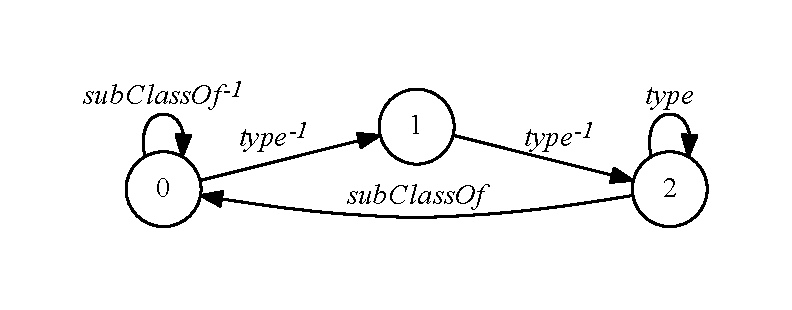
\includegraphics[width=8cm]{pictures/ExampleGraph.pdf}
	\]
	\caption{An input graph for the example query.}
	\label{ExampleQueryGraph}
\end{figure}

We provide a step-by-step demonstration of the work with the given graph $D$ and grammar $G'$ of the Algorithm~\ref{alg:graphParse}. After the matrix initialization in lines \textbf{6-7} of the Algorithm~\ref{alg:graphParse} we have a matrix $T_0$ presented in Figure~\ref{ExampleQueryInitMatrix}.

\begin{figure}[h]
	\[
	T_0 = \begin{pmatrix}
	\{S_1\} & \{S_3\} & \varnothing \\ \varnothing & \varnothing & \{S_3\} \\ \{S_2\} & \varnothing & \{S_4\}
	\end{pmatrix}
	\]
	\caption{Initial matrix for the example query.}
	\label{ExampleQueryInitMatrix}
\end{figure}

We denote $T_i$ as a matrix $T$ after $i$-th loop iteration in lines \textbf{8-9} of the Algorithm~\ref{alg:graphParse}. The calculation of the matrix $T_1$ is shown in Figure~\ref{ExampleQueryFirstIteration}.

\begin{figure}[h]
	\[
	T_0 \times T_0 = \begin{pmatrix}
	\varnothing & \varnothing & \varnothing \\ \varnothing & \varnothing & \{S\} \\ \varnothing & \varnothing & \varnothing
	\end{pmatrix}
	\]
	
	\[
	T_1 = T_0 \cup (T_0 \times T_0) = \begin{pmatrix}
	\{S_1\} & \{S_3\} & \varnothing \\ \varnothing & \varnothing & \{S_3, S\} \\ \{S_2\} & \varnothing & \{S_4\}
	\end{pmatrix}
	\]
	\caption{The first iteration of computing the transitive closure for the example query.}
	\label{ExampleQueryFirstIteration}
\end{figure}

When the algorithm at some iteration finds new paths in the graph $D$, then it adds corresponding nonterminals to the matrix $T$. For example, after the first loop iteration, nonterminal $S$ is added to the matrix $T$. This nonterminal is added to the element with a row index $i = 1$ and a column index $j = 2$. This means that there is $i\pi j$ (a path $\pi$ from node 1 to node 2), such that $S \xrightarrow{*} l(\pi)$. For example, such a path consists of two edges with labels $type^{-1}$ and $type$, and thus $S \xrightarrow{*} type^{-1} \ type$.

The calculation of the transitive closure is completed after $k$ iterations when a fixpoint is reached: $T_{k-1} = T_k$. For the example query, $k = 6$, since $T_6 = T_5$. The remaining iterations of computing the transitive closure are presented in Figure~\ref{ExampleQueryFinalIterations}.

\begin{figure}[h]
	\[
	T_2 = \begin{pmatrix}
	\{S_1\} & \{S_3\} & \varnothing \\ \{S_5\} & \varnothing & \{S_3, S, S_6\} \\ \{S_2\} & \varnothing & \{S_4\}
	\end{pmatrix}
	\]
	
	\[
	T_3 = \begin{pmatrix}
	\{S_1\} & \{S_3\} & \{S\} \\ \{S_5\} & \varnothing & \{S_3, S, S_6\} \\ \{S_2\} & \varnothing & \{S_4\}
	\end{pmatrix}
	\]
	
	\[
	T_4 = \begin{pmatrix}
	\{S_1, S_5\} & \{S_3\} & \{S, S_6\} \\ \{S_5\} & \varnothing & \{S_3, S, S_6\} \\ \{S_2\} & \varnothing & \{S_4\}
	\end{pmatrix}
	\]
	
	\[
	T_5 = \begin{pmatrix}
	\{S_1, S_5, S\} & \{S_3\} & \{S, S_6\} \\ \{S_5\} & \varnothing & \{S_3, S, S_6\} \\ \{S_2\} & \varnothing & \{S_4\}
	\end{pmatrix}
	\]
	\caption{Remaining states of the matrix $T$.}
	\label{ExampleQueryFinalIterations}
\end{figure}

Thus, the result of the Algorithm~\ref{alg:graphParse} for the example query is the matrix $T_5 = T_6$. Now, after constructing the transitive closure, we can construct the context-free relations $R_A$. These relations for each nonterminal of the grammar $G'$ are presented in Figure~\ref{ExampleQueryCFRelations}.

\begin{figure}[h]
	\begin{eqnarray*}
		R_S&=&\{(0,0),(0,2),(1,2)\},\\
		R_{S_1}&=&\{(0,0)\},\\
		R_{S_2}&=&\{(2,0)\}, \\
		R_{S_3}&=&\{(0,1), (1,2)\}, \\
		R_{S_4}&=&\{(2,2)\}, \\
		R_{S_5}&=&\{(0,0), (1,0)\}, \\
		R_{S_6}&=&\{(0,2), (1,2)\}.
	\end{eqnarray*}
	\caption{Context-free relations for the example query.}
	\label{ExampleQueryCFRelations}
\end{figure}

By the context-free relation $R_S$, we can conclude that there are paths in a graph $D$ only from node 0 to node 0, from node 0 to node 2 or from node 1 to node 2, corresponding to the context-free grammar $G_S$. This conclusion is based on the fact that a grammar $G'_S$ is equivalent to the grammar $G_S$ and $L(G_S) = L(G_S')$. The result of the all-pairs CFL-reachability analysis for this example is a set of node pairs $R_S$.


\section{Conclusion and Future Work}%--------------------------------------------------------------------------------------------------------------------------------------------
In this paper, we shown how the all-pairs CFL-reachability problem can be reduced to the calculation of the matrix transitive closure. Also, we introduced an algorithm for computing this transitive closure. Finally, we provided a formal proof of the correctness of the proposed algorithm and show that the worst-case time complexity of this algorithm is $O(n^2BMM(n))$.

We can identify several open problems for further research. In this paper we have considered only one formulation of the CFL-reachability analysis but there are other important formulations~\cite{hellingsPathQuerying} which requires to present some path for all node pairs $(m,n)$. Our algorithm can be modified to store path lengths associated with each nonterminal in the matrix. The required path of a fixed length for all node pairs $(m,n)$ can be found by a simple search and checking whether the labels of this path form a string which is generated by the given context-free grammar.

In our algorithm, we calculate the matrix transitive closure naively, but there are algorithms for the transitive closure calculation, which are asymptotically more efficient. Therefore, the question is whether it is possible to apply these algorithms for the matrix transitive closure calculation to the graph reachability problems. The main problem in this area is to reduce this transitive closure calculation to exactly one Boolean matrix multiplication and solve the all-pairs CFL-reachability problem in less than cubic time. 

Also, there are conjunctive~\cite{okhotinConjAndBool} and Boolean grammars~\cite{okhotinBoolean}, which have more expressive power than context-free grammars. Conjunctive language and Boolean path querying problems are undecidable~\cite{hellingsRelational} but our algorithm can be trivially generalized to work on this grammars because parsing with conjunctive and Boolean grammars can be expressed by matrix multiplication~\cite{okhotin_cyk}. It is not clear what a result of our algorithm applied to this grammars would look like. Our hypothesis is that it would produce the upper approximation of a solution. Also, graph reachability problem w.r.t. the conjunctive grammars can be applied to static code analysis~\cite{zhang2017context}.

From a practical point of view, matrix multiplication in the main loop of the proposed algorithm can be effectively calculated using such computing techniques as GPGPU (General-Purpose computing on Graphics Processing Units) and parallel computation. This matrix operations may be performed on different GPGPU independently. It can help to utilize the power of multi-GPU systems and increase the performance of the context-free path querying. Also, a sparse matrix representation can be used to increase performance on the large graphs.

\section*{Acknowledgments}%--------------------------------------------------------------------------------------------------------------------------------------------

We are grateful to Dmitri Boulytchev, Ekaterina Verbitskaia, Marina Polubelova, Dmitrii Kosarev and Dmitry Koznov for their careful reading, pointing out some mistakes, and invaluable suggestions.
This work is supported by grant from JetBrains Research.

\bibliographystyle{abbrv}
\bibliography{bibliography}
\section{Dataset description}\label{section:dataset}

In our evaluation we use dataset which contains the following parts.
{\setlength{\tabcolsep}{0.4em}
	\begin{table}[h]
		\caption{RDFs properties}
		\label{tbl:propRDF}
		\rowcolors{2}{}{lightgray}
		\begin{tabular}{| l | c | c | c | c |}
			\hline
			Name                  & \#V    & \#E     & \#type &\#subClassOf \\
			\hline
			\hline
			atom-primitive				& 291		& 685		& 138	& 122	\\
			univ-bench					& 179		& 413		& 84		& 36		\\
			travel						& 131		& 397		& 90		& 30		\\
			skos							& 144		& 323		& 70		& 1		\\
			people\_pets					& 337		& 834		& 161	& 33		\\
			generations					& 129		& 351		& 78		& 0		\\
			foaf							& 256		& 815		& 174	& 10		\\
			biomed-mesure-prim   	    & 341		& 711		& 130	& 122	\\
			funding						& 778		& 1480		& 304	& 90               \\
			pizza						& 671		& 2604		& 365	& 259              \\
			wine							& 733		& 2450		& 485	& 126              \\
			core							& 1323		& 8684		& 1412	& 178              \\
			pathways						& 6238		& 37196		& 3118 	& 3117             \\
			go-hierarchy					& 45007		& 1960436	& 0		& 490109           \\
			enzyme						& 48815		& 219390		& 14989	& 8163             \\
			eclass\_514en				& 239111		& 1047454	& 72517	& 90962            \\
			go							& 272770		& 1068622	& 58483	& 90512            \\
			\hline
		\end{tabular}
	\end{table}
}

{\setlength{\tabcolsep}{0.4em}
\begin{table*}[h]
\caption{RDFs query $G_2$ (time is measured in seconds and memory is measured in megabytes)}
\label{tbl:tableRDFQ2}
\rowcolors{3}{}{lightgray}
\begin{tabular}{| l | r  r | r  r | r  r | r  r | r  r |}
    \hline

    \multirow{3}{*}{Name}   &   \multicolumn{6}{|c|}{Relational semantics index}	&	\multicolumn{4}{|c|}{Single path semantics index} \\
    \cline{2-11}
    &	\multicolumn{2}{|c|}{RG\_CPU\textsubscript{rel}}	&	\multicolumn{2}{|c|}{RG\_CUSP\textsubscript{rel}}	&	\multicolumn{2}{|c|}{RG\_SPARSE\textsubscript{rel}} &	\multicolumn{2}{|c|}{RG\_CPU\textsubscript{path}}	&	\multicolumn{2}{|c|}{RG\_SPARSE\textsubscript{path}}	 \\
    \cline{2-11}
    &   Time & Mem &  Time     & Mem & Time     & Mem  &  Time     & Mem & Time     & Mem \\
    \hline
    \hline
    atom-primitive          & 0.001 & 0.3  & 0.001 & 0.1 & 0.002 & 0.1   & 0.001 & 0.3  & 0.002 & 0.1   \\
biomedical-mesure-primitive & 0.002 & 0.1  & 0.014 & 2.0   & 0.009 & 0.1   & 0.006 & 0.1  & 0.012 & 0.1   \\
core                        & 0.001 & 0.3  & 0.006 & 0.1 & 0.004 & 0.1   & 0.003 & 0.3  & 0.005 & 0.1   \\
eclass\_514en               & 0.035 & 6.5  & 0.020 & 16.0  & 0.100   & 12.0    & 0.123 & 17.7 & 0.127 & 18.0    \\
enzyme                      & 0.006 & 3.9  & 0.006 & 0.6 & 0.010  & 0.1   & 0.012 & 5.3  & 0.008 & 0.4   \\
foaf                        & 0.001 & 0.1  & 0.004 & 0.1 & 0.002 & 0.1   & 0.001 & 0.1  & 0.003 & 0.1   \\
funding                     & 0.002 & 0.1  & 0.015 & 0.4 & 0.007 & 0.1   & 0.009 & 0.1  & 0.008 & 0.1   \\
generations                 & 0.001 & 0.1  & 0.001 & 0.1 & 0.001 & 0.1   & 0.001 & 0.1  & 0.001 & 0.1   \\
go-hierarchy                & 0.095 & 17.8 & 0.253 & 528.0 & 0.175 & 130.4 & 0.884 & 88.8 & 0.306 & 138.8 \\
go                          & 0.306 & 25.8 & 0.240 & 84.0  & 0.181 & 25.4  & 0.918 & 78.1 & 0.219 & 34.2  \\
pathways                    & 0.005 & 0.2  & 0.005 & 0.4 & 0.004 & 0.1   & 0.017 & 0.5  & 0.003 & 0.1   \\
people\_pets                & 0.001 & 0.1  & 0.007 & 0.1 & 0.004 & 0.1   & 0.001 & 0.1  & 0.005 & 0.1   \\
pizza                       & 0.002 & 0.3  & 0.012 & 0.2 & 0.008 & 0.1   & 0.010  & 0.3  & 0.009 & 0.1   \\
skos                        & 0.001 & 0.1  & 0.001 & 0.1 & 0.001 & 0.1   & 0.001 & 0.1  & 0.002 & 0.1   \\
travel                      & 0.001 & 0.1  & 0.007 & 0.1 & 0.005 & 0.1   & 0.001 & 0.1  & 0.005 & 0.1   \\
univ-bench                  & 0.001 & 0.1  & 0.007 & 0.1 & 0.005 & 0.1   & 0.001 & 0.1  & 0.005 & 0.1   \\
wine                        & 0.001 & 0.3  & 0.006 & 0.1 & 0.004 & 0.1   & 0.002 & 0.3  & 0.004 & 0.1  \\
    \hline
  \end{tabular}
\end{table*}
}

\begin{itemize}
\item The real-world data RDFs provided in CFPQ\_Data dataset\footnote{CFPQ\_Data dataset GitHub repository: \url{https://github.com/JetBrains-Research/CFPQ_Data}. Access date: 12.11.2019.} from~\cite{Mishin:2019:ECP:3327964.3328503}.
\item Geospecies (RDF which contains information about biological hierrarchy\footnote{The Geospecies RDF: \url{https://old.datahub.io/dataset/geospecies}. Access date: 12.11.2019.} and same-generation query over \textit{broaderTransitive} relation) is provided in~\cite{Kuijpers:2019:ESC:3335783.3335791} and integrated in our evaluation with CFPQ\_Data.
\item It was shown in~\cite{Mishin:2019:ECP:3327964.3328503} that matrix-based algorithm is performant enough to handle bigger RDFs than those used in the initial datasets, such as~\cite{RDF}.
So, we add several big RDFs to CFPQ\_Data and use them in our evaluation.
New RDFs: \textit{go-hierarchy, go, enzime, core, pathways} are from UniProt database\footnote{Protein sequences data base: \url{https://www.uniprot.org/}. RDFs with data are avalable here: \url{ftp://ftp.uniprot.org/pub/databases/uniprot/current_release/rdf}. Access date: 12.11.2019}, and \textit{eclass-514en} is from eClassOWL project\footnote{eClassOWL project: \url{http://www.heppnetz.de/projects/eclassowl/}. eclass-514en file is available here: \url{http://www.ebusiness-unibw.org/ontologies/eclass/5.1.4/eclass_514en.owl}. Access date: 12.11.2019.}.
\end{itemize}

The properties of the RDFs from the dataset are given in table \ref{tbl:propRDF}. 
Geospecies RDF contains 450609 vertices, 2311461 edges, and 20867 edges labeled by \textit{broaderTransitive}.
Note that while the number of edges labeled by \textit{broaderTransitive} is equal to provided in~\cite{Kuijpers:2019:ESC:3335783.3335791}, the total number of vertices and edges is bigger. It is because we naively convert each triple from RDF to edge in the graph, while J. Kuijpers et al. use special \textit{neosemantics}\footnote{Neosemantix is an RDF processing plugin for Neo4j. Web page: \url{https://neo4j.com/labs/nsmtx-rdf/}. Access date: 30.03.2020.} plugin which can, for example, handling multivalued properties accurately.  

The variants of the \textit{same-generation query}~\cite{FndDB} are used in almost all cases because it is an important example of real-world queries that are context-free but not regular.
So, variations of the same generation query are used in our evaluation.
All queries are added to the CFPQ\_Data dataset.

We use two queries over \textit{subClassOf} and \textit{type} relations.
The first query is the grammar $G_1$:
\[
 \begin{array}{lcl}
   s  \rightarrow \textit{subClassOf}^{\ -1} \ s \ \textit{subClassOf}   & \quad & s  \rightarrow \textit{type}^{\ -1} \ s \ \textit{type}     \\
   s  \rightarrow \textit{subClassOf}^{\ -1} \ \textit{subClassOf}       & \quad & s  \rightarrow  \textit{type}^{\ -1}  \ \textit{type}

 \end{array}
 \]
The second one is the grammar $G_2$: \[s \rightarrow \textit{subClassOf}^{\ -1} \ s \ \textit{subClassOf} \mid \textit{subClassOf}\]

For geospecies we use same-generation query \textit{geo} from the original paper~\cite{Kuijpers:2019:ESC:3335783.3335791}: \[s \rightarrow \textit{broaderTransitive} \ s \ \textit{broaderTransitive}^{\ -1} \]
\[s \rightarrow \textit{broaderTransitive}  \ \textit{broaderTransitive}^{\ -1} \]


\section{Evaluation Details}

Results for RDFs querying with $G_2$ grammar are presented in table~\ref{tbl:tableRDFQ2}.
We can see, that for small graphs time for both relational and single-path querying are similar for CPU and GPGPU versions, but for bigger graphs (\textit{go} and \textit{go-hierarchy}, for example) GPUPU version is more performant than CPU one.

\balance


\end{document}
